\begin{definition}[Traceability~\cite{endrullis2024generalized}]
    \label{def:traceability}
    \ \newline
\noindent 
\begin{minipage}{0.5\textwidth}
An object $X \in \mathcal{C}$ is called \emph{traceable} along a class of pushout squares $\Delta$ if for every diagram $\delta \in \Delta$ (shown on the right), the following hold
\end{minipage}
\begin{minipage}{0.5\textwidth}
\begin{center}
    \begin{tikzpicture}[node distance=12mm]
      \node (A) {$A$};
      \node [right of=A] (B) {$B$}; 
      \node [below of=A] (C) {$C$}; 
      \node [below of=B] (D) {$D$}; 
      \node [right of=D] (X) {$X$};
      \begin{scope}[nodes=rectangle]          
      \draw [->] (A) to node [above,label,pos=0.5] {$\alpha$} (B);
      \draw [->] (A) to node [left,label,pos=0.5] {$\beta$} (C);
      \draw [->] (B) to node [right,label,pos=0.45] {$\beta'$} (D); 
      \draw [->] (C) to node [below,label,pos=0.45] {$\alpha'$} (D);
      \draw [->] (X) to node [below,label,pos=0.4] {$h$} (D);
      \end{scope}
      \node at ($(A)!.5!(D)$) {$\delta$};
    \end{tikzpicture}
\end{center}
\end{minipage}
    \begin{enumerate}[label=(\alph*)]
        \item\label{traceable:a} there exists a morphism $f : X \to B$ such that $h = f \star \beta'$, or
        \item\label{traceable:b} there exists a morphism $g : X \to C$ such that $h = g \star \alpha'$.
    \end{enumerate}
    If additionally, 
    \trackedtext{whenever \ref{traceable:a} and \ref {traceable:b} hold,} \todo{This starts to be quite hard to follow without intuition or example}
    \begin{enumerate}[label=(\alph*),resume]
        \item 
        there exists a morphism $k : X \to A$ such that $h = k \star \alpha \star \beta' $,
    \end{enumerate}
    then we say that $X$ is \emph{$\beta$-strongly traceable} along $\Delta$.
\end{definition}

Consider the category \textbf{Graph}. Intuitively, a graph $X$ is $\beta$-strongly traceable along a pushout squares as illustrated above, if whenever $X$ occurs in $D$, it occurs either in $B$ or in $C$, and if it occurs in both, then it occurs in $A$ as well.

\begin{example}
    Consider the DPO diagram in Example~\ref{ex:rewriting_step_grs_aa}. The graph \tikz[baseline=-0.5ex]{
        \node (x) at (0,0) {$\bullet$};
        \node (y) at (1,0) {$\bullet$};
        \node (z) at (2,0) {$\bullet$};
        \draw[->] (x) -- (y) node[midway, above] {$a$};
        \draw[<-] (z) -- (y) node[midway, above] {$a$};
    } is not traceable in both pushout squares. The graph \tikz[baseline=-0.5ex]{
        \node (x) at (0,0) {$\bullet$};
        \node (y) at (1,0) {$\bullet$};
        \draw[->] (x) -- (y) node[midway, above] {$a$};
    } is traceable (and strongly traceable) along both pushout squares.
\end{example}

\begin{example}
    The graph 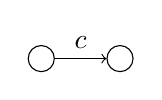
\begin{tikzpicture}
        \node[draw, circle] (x) at (0,0) {};
        \node[draw, circle] (y) at (1,0) {};
        \draw[->]  (x) -- (y) node [midway,above] {$c$};
    \end{tikzpicture} 
    is traceable along both pushout squares. 
     It is $u$-strongly traceable along the left pushout square, but not $u$-strongly traceable along the right pushout square. 
    The graph 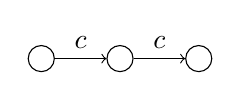
\begin{tikzpicture}
        \node[draw, circle] (x) at (0,0) {};
        \node[draw, circle] (y) at (1,0) {};
        \node[draw, circle] (z) at (2,0) {};
        \draw[->]  (x) -- (y) node [midway,above] {$c$};
        \draw[->]  (y) -- (z) node [midway,above] {$c$};
    \end{tikzpicture} is not traceable along both pushout squares.
%     because    
%     \begin{tikzpicture}
%        \node[draw, circle] (x) at (0,0) {z};
%        \node[draw, circle] (y) at (1,0) {x};
%        \node[draw, circle] (z) at (2,0) {y};
%        \draw[->]  (x) -- (y) node [midway,above] {$c$};
%        \draw[->]  (y) -- (z) node [midway,above] {$c$};
%    \end{tikzpicture} is in the pushout object $G$ but in neither $L$ nor $C$.

    \resizebox{0.7\textwidth}{!}{
    \begin{tikzpicture}
        \graphbox{$L$}{0mm}{0mm}{35mm}{35mm}{2mm}{-5mm}{
        \node[draw,circle] (1) at (0,0) {x};
        \node[draw,circle] (2) at (1,-2) {y};
        \node[draw,circle] (3) at (-1,-2) {z};
        \draw[->] (1) edge node[midway,right]  {$c$}  node[midway,left]{} (2);
        \draw[->] (2) edge node[midway,above]  {$c$}  node[midway,below]{}  (3);
        }
        \graphbox{$K$}{45mm}{0mm}{35mm}{35mm}{2mm}{-5mm}{
        % I
            % \def\x{5};
            % \def\y{0};
            \node[draw,circle] (1) at (0,0) {x};
            \node[draw,circle] (2) at (1,-2) {y};
            \node[draw,circle] (3) at (-1,-2) {z};
            \draw[->] (2) edge node[midway,above]  {$c$}  node[midway,below]{}  (3);
        }
        \node () at (40mm,-15mm)  {$\overset{l}{\leftarrowtail}$};

        % \node () at (2.5,-2.5) {$PO$};
        \graphbox{$R$}{90mm}{0mm}{35mm}{35mm}{2mm}{-5mm}{
        % R
            % \def\x{10};
            % \def\y{-1.1};
            \node[draw,circle] (1) at (0,-1) {x y z};
            \draw[->] (1) edge[loop below]  node[midway, above] {$c$}  node[midway, below] {} (1);
        }
        \node () at (85mm,-15mm)  {$\overset{r}{\rightarrow}$};

        \graphbox{$G$}{0mm}{-45mm}{35mm}{35mm}{2mm}{-5mm}{
        % \node () at (7.5,-2.5) {$PO$};
        % G
            % \def\x{0};
            % \def\y{-5};
            \node[draw,circle] (1) at (0,0) {x};
            \node[draw,circle] (2) at (1,-2) {y};
            \node[draw,circle] (3) at (-1,-2) {z};
            \draw[->] (1) edge node[midway,right]  {$c$}  node[midway,left]{} (2);
            \draw[->] (2) edge node[midway,above]  {$c$}  node[midway,below]{}  (3);
            \draw[->] (3) edge node[midway,above]  {$c$}  node[midway,below]{}  (1);
        }
        % C
        \graphbox{$C$}{45mm}{-45mm}{35mm}{35mm}{2mm}{-5mm}
        {    
            \node[draw,circle] (1) at (0,0) {x};
            \node[draw,circle] (2) at (1,-2) {y};
            \node[draw,circle] (3) at (-1,-2) {z};
            % \draw[->] (1) edge node[midway,right]  {$c$}  node[midway,left]{} (2);
            \draw[->] (3) edge node[midway,above]  {$c$}  node[midway,below]{} (1);
            \draw[->] (2) edge node[midway,above]  {$c$}  node[midway,below]{} (3);
            }
        \node () at (40mm,-55mm)  {$\overset{l}{\leftarrowtail}$};
        % H
        \graphbox{$H$}{90mm}{-45mm}{35mm}{35mm}{2mm}{-5mm}{
        % R
            % \def\x{10};
            % \def\y{-1.1};
            \node[draw,circle] (1) at (0,-1) {x y z};
            \draw[->] (1) edge[loop below]  node[midway, below] {} node[midway, above] {$c$} (1);
            \draw[->] (1) edge[loop above]  node[midway, below] {} node[midway, above] {$c$} (1);
        }

        \node () at (85mm,-55mm)  {$\overset{r}{\rightarrow}$};
        \node () at (17mm,-40mm) {$m\downarrowtail$};
        \node () at (62mm,-40mm) {$u\downarrowtail$};
        \node () at (107mm,-40mm) {$\downarrow m'$};
    \end{tikzpicture}
    }
\end{example} 